% write your paper in here

\chapter{Genome assembly of a chaetognath}

\section{Introduction}

Chaetognaths, commonly known as arrow worms, are transparent marine predators widely distributed at various depths in all oceans, though low depth remains the favorite habitat of most species  \cite{alvarino1964bathymetric}. They are characterized by a transparent and elongated body, with one or two pairs of lateral fins, a caudal fin, a head with hooks, and range in size from a few millimeters to several centimeters \cite{ghirardelli1969}. Current chaetognath species are divided into two orders depending on the presence of transversal muscles, or phragms: Phragmophora and Aphragmophora \cite{tokioka1965taxonomical}. The whole phylum now encompasses about 150 species. They form an enigmatic clade whose phylogenetic position is still discussed. Chaetognaths were initially considered as deuterostomians, due to their development, but analyses of 18S rDNA rejected this hypothesis \cite{telford1993phylogenetic,wada1994details} and further brought support to the Phragmophora and Aphragmophora branches \cite{telford1997evolution}. Later, Nielsen suggested that chaetognaths belonged to the clade Gnathifera \cite{nielsen2011}, which gathers Gnathostomulida, Micrognathozoa and Rotifera. This hypothesis was supported by a recent transcriptome analysis of ten chaetognath species \cite{marletaz2019new}.  \\

To this day, there is no genome assembly available for the whole phylum Chaetognatha, despite the fact that such a resource could help resolve and refine their phylogenetic position. Within the framework of the IGNITE consortium and my PhD project, I therefore tackled the assembly of a chaetognath genome, provisionally identified as \textit{Flaccisagitta enflata} (see below). This species was first described by Grassi in 1881; it belongs to the order Aphragmophora and the family Sagittidae. It is epipelagic and present across all oceans in warmer waters \cite{michel1984}. This species was selected based on specimen sizes (up to 2.5 cm), to avoid pooling individuals for sequencing and running into more haplotyping complexity, and its moderate genome size, estimated at 0.71 pg \cite{animal_genome_size}. \\

\section{Material \& Method}

\subsection{Collection and fixation}

Chaetognaths were collected by Mark Vermeij around the island of Curaçao after sunset from October 29th to November 2nd 2019. A total of 30 individuals were sampled: eleven were crosslinked in 3\% formaldehyde for 30 to 45 minutes, quenched in 250 mM glycine, then frozen at -80{\degree}C; twelve were preserved in absolute ethanol and kept at 4{\degree}C; seven were preserved in RNAlater and kept at 4{\degree}C. All samples used for DNA, RNA and Hi-C sequencing were collected on November 2nd 2019 in Snake Bay.

\subsection{High-molecular-weight DNA extraction}

One 2-cm individual preserved in ethanol was incubated in 180 {\textmu}L of CTAB buffer (described in Table \ref{tab:ctab}) and 25 {\textmu}L of proteinase K for 3 hours at 60{\degree}C and 300 rpm. The lysed sample was purified with phenol-chloroform-isoamyl alcohol 25:24:1, chloroform-isoamyl alcohol 24:1 and with AMPure XP beads. I obtained 2.5 {\textmu}g of DNA with OD260/280 = 1.95 and OD260/230 = 1.95.

\begin{table}[H]
\centering
\caption{Composition of the cetyltrimethylammonium bromide (CTAB) buffer.}
\begin{tabular}{|l|l|l|}
\hline
\textbf{Solution} & \textbf{Stock concentration} & \textbf{Volume for 2.45 mL} \\
\hline
Polyvinylpyrrolidone (PVP) & 10\% & 500 {\textmu}L \\
Tris(hydroxymethyl)aminomethane-HCl & 1 M & 250 {\textmu}L \\
Ethylenediaminetetraacetic acid (EDTA) & 500 mM & 125 {\textmu}L \\
NaCl & 5 M & 1 mL \\
H\textsubscript{2}O & - & 75 {\textmu}L \\
CTAB & 10\% & 500 {\textmu}L \\
{\textbeta}-mercaptoethanol & - & 25 {\textmu}L \\
\hline
\end{tabular}
\label{tab:ctab}
\end{table}

\subsection{Whole-genome sequencing}

The library for Nanopore sequencing was prepared with the Nanopore SQK-LSK109 Ligation sequencing kit. This library was loaded four times in the PromethION flow cell with nuclease flushes in between. The flow cell (with pore proteins R9.4.1) ran for 72 hours and gave an output of 40.5 Gb with an N50 = 6.1 kb. Basecalling was done with Guppy v4. 168 Gb of paired-end 150-bp Illumina reads were also sequenced by Novogene.

%\begin{figure}[H]
%    \centering
%    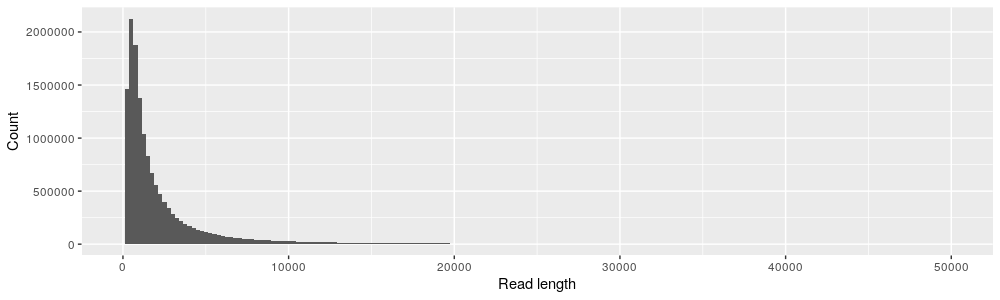
\includegraphics[width=0.9\linewidth]{fig/fenflata_ONT_read_length_distribution.png}
%    \caption{Read length distribution of Nanopore reads up to 50 kb (bin = 500 bases).}
%    \label{fig:histo_ONT}
%\end{figure}

%\subsection{RNA extraction and sequencing}

%One 1.2-cm individual preserved in RNAlater was mixed in 1 mL Trizol. Then the sample was purified with 200 {\textmu}L of chloroform-isoamyl alcohol, and the RNA was recovered using 500 {\textmu}L of isopropanol. With this protocol, I obtained 3.4 {\textmu}g of RNA with OD260/280 = 1.79 and OD260/230 = 1.95. The cDNA sequencing library was prepared using the Nanopore PCR-cDNA sequencing kit and was sequenced using a MinION flow cell, which yielded 909 Mb and 1.98 million reads. RNA was also extracted from another 1.8-cm individual preserved in RNAlater by Novogene, using a similar Trizol-based protocol. This sample was sequenced on a NovaSeq platform and yielded 201 millions pairs of reads of 150 bases. 

\subsection{Hi-C sequencing}

One 1.5-cm individual crosslinked in 3\% formaldehyde was used to prepare a Hi-C library with the Arima Hi-C kit (including the restriction enzymes DpnII and HinfI), and resulted in 466 ng of DNA. The DNA was fragmented with a Covaris (300 bp) and biotinylated fragments were selected with streptavidin beads. The library was prepared for Illumina sequencing using Invitrogen TM Collibri TM PS DNA Library Prep Kit and following manufacturer instructions. Sequencing by Novogene resulted in 489 millions pairs of reads of 150 bp.

\subsection{Pre-assembly analysis}

The genome size was estimated with BBtools \cite{bbtools} using the script \texttt{kmercountexact.sh} and the shotgun Illumina reads. As this tool is based on \textit{k}-mers, three values of \textit{k} were tested with \textit{k} = \{27, 29, 31\}. A \textit{k}-mer histogram of the Illumina dataset was built using KAT hist v2.4.2 (with \textit{k} = 27). 

\subsection{Genome assembly}

The Nanopore reads were trimmed using Porechop \cite{porechop} with default parameters, then they were assembled \textit{de novo} with several assemblers: Canu \cite{canu}, Flye \cite{flye}, Ra \cite{ra}, Raven \cite{raven} and wtdbg2 \cite{wtdbg2}. The assemblies were polished with HyPo \cite{hypo} and remaining uncollapsed haplotypes were purged with purge\_dups \cite{purge_dups} and Purge Haplotigs \cite{purge_haplotigs}. I also tried preprocessing the reads by filtering them using a length threshold or the tool Filtlong with the parameters \texttt{-{}-keep\_percent 52.0 -{}-min\_length 2000}. Assembly pipelines were defined following the strategies identified in Chapter 2. Two assemblies were selected as candidates for Hi-C scaffolding:
\begin{itemize}
    \item[--] FEv1: Ratatosk + Canu + purge\_dups x2
    \item[--] FEv2: Raven + HyPo + purge\_dups + Purge Haplotigs
\end{itemize}

\subsection{Hi-C scaffolding}

Hi-C reads were mapped to the draft assemblies using hicstuff \cite{hicstuff} with the parameters \texttt{-{}-enzyme DpnII,HinfI -{}-aligner bowtie2 -{}-iterative}. instaGRAAL was run with the parameters \texttt{-{}-level 5 -{}-cycles 150}. The scaffolds were post-processed with instaGRAAL-polish to reduce misassemblies and 10 Ns were added as gaps.

\subsection{Gap filling}

Gaps in the scaffolded assemblies were filled by TGS-GapCloser \cite{tgsgapcloser} using the Ratatosk-corrected Nanopore reads for FEv1 and the Nanopore reads for FEv2. FEv1 was further polished using HyPo. 

\subsection{Assembly evaluation}

Assemblies were assessed using BUSCO v4 against the lineage metazoa odb10 without the parameter \texttt{-{}-long} and using KAT comp 2.4.2 against the Illumina dataset (with \textit{k} = 27. Contact maps were built for scaffolded assemblies using the hicstuff pipeline as described previously and hicstuff view with the parameter \texttt{-{}-binning 2000}.

\section{Results}

\subsection{Species identification}

Morphological characteristics were registered in living and fixed individuals in order to identify the species: 
\begin{itemize}
    \item[--] length up to 2.5 cm;
    \item[--] body transparent, soft and inflated-looking;
    \item[--] 8-10 hooks (Figure 1.A1);
    \item[--] no collarette;
    \item[--] anterior position of the ganglion (Figure 1.A2);
    \item[--] pair of lateral fins;
    \item[--] short rounded fins;
    \item[--] ovaries not extending till the anterior fins (Figure 1.B3);
    \item[--] round vesicles close to the tail (Figure 1.B4).
\end{itemize}

\begin{figure}[H]
    \centering
    \includegraphics[width=0.9\linewidth]{fig/rect1951.png}
    \caption{A chaetognath specimen fixed in 3\% formaldehyde. This individual was used for Hi-C sequencing.}
\end{figure}

The specimens were all provisionally identified as \textit{Flaccisagitta enflata} using the identification key provided in Michel \cite{michel1984}. 

\subsection{Whole-genome assembly}

The haploid genome size was estimated to 695-699 Mb, which matches the estimation available on the Animal Genome Size Database \cite{animal_genome_size} of 0.71 picograms (approximately 694 Mb), measured with Feulgen densitometry. The \textit{k}-mer histogram shows two distinct peaks, one around 85X, for heterozygous \textit{k}-mers, and a second around 172X, for homozygous \textit{k}-mers, thus the genome is diploid (Figure \ref{fig:fenflata_kat_hist}). The homozygous peak is strikingly small compared to the heterozygous peak, indicating a high level of heterozygosity. 

\begin{figure}
    \centering
    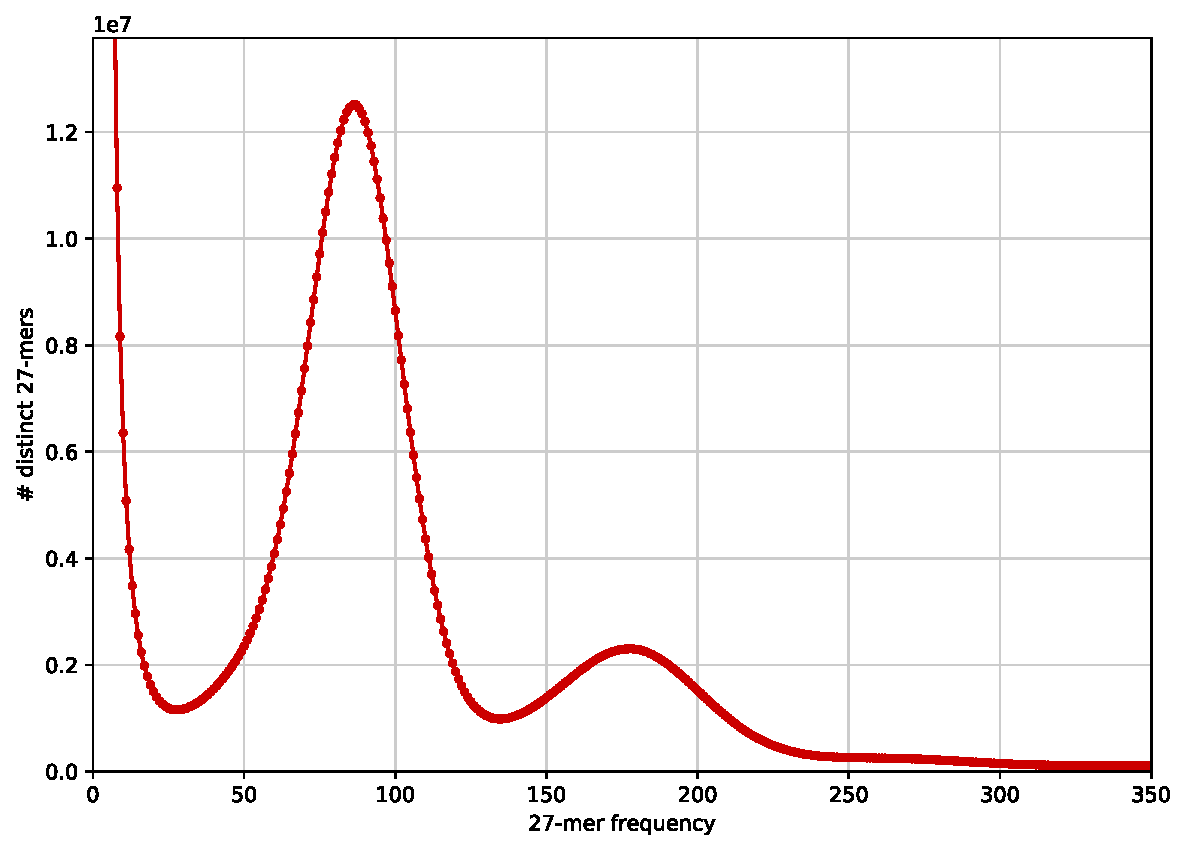
\includegraphics[width=1\linewidth]{fig/fenflata_kat_illumina.eps}
    \caption{\textit{k}-mer analysis of the Illumina dataset.}
    \label{fig:fenflata_kat_hist}
\end{figure}

Most initial assemblies had a size larger than the expected genome size (Table \ref{tab:chaeto_assemblies}), due to the high heterozygosity of the genome that leads to artefactual duplications, as described in Chapter 2. Canu and Flye tend to retain uncollapsed haplotypes; Flye yielded an assembly about twice the expected haploid size when using all raw Nanopore reads (1.45 Gb), suggesting a diploid assembly, but surprisingly Canu produced a smaller assembly than expected (614 Mb). These behaviors were reversed with the Ratatosk-corrected Nanopore dataset: the Canu assembly was likely diploid (1.48 Gb), while the Flye assembly was close to the haploid genome size (849 Mb). However, the poor BUSCO score of the Ratatosk-Flye assembly suggested that it was not a good candidate. Two rounds of purge\_dups greatly improved the Canu-Ratatosk and Flye-HyPo assemblies, as the number of duplicated BUSCO features were reduced in favor of single-copy BUSCO features. The Ratatosk-Canu-purge\_dups assembly (designated as FEv1) was selected for scaffolding based on its high BUSCO score, low duplicated features and contiguity. The Ra assembly of raw Nanopore reads longer than 5 kb was the closest to the expected genome size (728 Mb), yet the BUSCO score after polishing is low (80.4\% single-copy and duplicated features). The Raven assembly of all raw reads was oversized, and after polishing the BUSCO score pointed at a large amount of duplications (30.9\% duplicated features). A combination of purge\_dups and Purge Haplotigs diminished the number of duplicated features (11.6\%) and increased the single-copy BUSCO score (78.9\%); this assembly was selected for scaffolding as FEv2. The wtdbg2 assembly had a moderate amount of duplications, but its BUSCO completeness after polishing was still lower than FEv1 and FEv2.

\begin{table}
\centering
\caption{Assembly statistics. purge\_dups and Purge Haplotigs are respectively designated as PD and PH.}
\resizebox{\columnwidth}{!}{
\begin{tabular}{lccccccccccc}
   \hline
    \multirow{2}{*}{\textbf{Assembly}} & \textbf{Read} & \textbf{Hybrid} & \multirow{2}{*}{\textbf{Polishing}} & \textbf{Haplotig} & \textbf{Assembly} & \multirow{2}{*}{\textbf{\# contigs}} & \multirow{2}{*}{\textbf{N50}} & \textbf{Largest} & \multicolumn{2}{c}{\textbf{BUSCO}} \\
        & \textbf{selection} & \textbf{correction} &  & \textbf{purging} & \textbf{size} &  &  & \textbf{contig} & \textbf{single} & \textbf{dup.} \\
    \hline
    Canu & 5 kb & $\times$ & $\times$ & $\times$ & 614 Mb & 24038 & 44 kb & 497 kb & 27.6\% & 2.7\% \\
        & $\times$ & Ratatosk & $\times$ & $\times$ & 1.48 Gb & 13385 & 195 kb & 1.2 Mb & 28.3\% & 66.0\% \\
        & $\times$ & Ratatosk & $\times$ & PD x2 & 946 Mb & 9288 & 215 kb & 1.2 Mb & 85.4\% & 7.1\% \\
    \hline
    Flye & $\times$ & $\times$ & $\times$ & $\times$ & 1.45 Gb & 31205 & 264 kb & 1.6 Mb & 61.1\% & 12.3\% \\
        & $\times$ & Ratatosk & $\times$ & $\times$ & 849 Mb & 40273 & 50 kb & 967 kb & 43.9\% & 47.1\% \\
        & $\times$ & $\times$ & HyPo & $\times$ & 1.45 Gb & 31205 & 263 kb & 1.6 Mb & 35.0\% & 58.8\% \\
        & $\times$ & $\times$ & HyPo & PD x2 & 985 Mb & 9508 & 277 kb & 1.6 Mb & 71.2\% & 19.8\% \\
    \hline
    Ra & 5 kb & $\times$ & $\times$ & $\times$ & 728 Mb & 7706 & 110 kb & 509 kb & 42.9\% & 1.3\% \\
        & 5 kb & $\times$ & HyPo & $\times$ & 730 Mb & 7706 & 111 kb & 510 kb & 68.8\% & 11.6\% \\
        & Filtlong & $\times$ & $\times$ & $\times$ & 684 Mb & 7507 & 106 kb & 498 kb & 39.7\% & 0.6\% \\
    \hline
    Raven & $\times$ & $\times$ & $\times$ & $\times$ & 1.10 Gb & 7656 & 185 kb & 1.2 Mb & 60.0\% & 6.0\% \\
        & 5 kb & $\times$ & $\times$ & $\times$ & 1.01 Gb & 6901 & 180 kb & 864 kb & 37.8\% & 0.9\% \\
        & Filtlong & $\times$ & $\times$ & $\times$ & 1.01 Gb & 6741 & 186 kb & 1.0 Mb & 36.3\% & 1.3\% \\
        & $\times$ & $\times$ & HyPo & $\times$ & 1.10 Gb & 7656 & 186 kb & 1.2 Mb & 61.1\% & 30.9\% \\
        & $\times$ & $\times$ & HyPo & PD + PH & 929 Mb & 6612 & 191 kb & 1.2 Mb & 78.9\% & 11.6\% \\
    \hline
    wtdbg2 & $\times$ & $\times$ & $\times$ & $\times$ & 965 Mb & 13558 & 219 kb & 2.0 Mb & 19.3\% & 0.2\% \\
        & $\times$ & $\times$ & HyPo & $\times$ & 987 Mb & 13558 & 224 kb & 2.1 Mb & 71.5\% & 13.1\% \\
    \hline
\end{tabular}
}
\label{tab:chaeto_assemblies}
\end{table}

The mapping rate of Hi-C reads was low for both FEv1 and FEv2: only 37\% of the reads aligned unambiguously. Scaffolding with instaGRAAL yielded 9 chromosome-level scaffolds (Table \ref{tab:chaeto_scaffolded_assemblies}, Figure \ref{fig:fenflata_contact_maps}) that were retained for the final assemblies, to discard contamination from bacteria and plankton in the digestive tube. The cumulative sizes of the 9 scaffolds are close to the expected genome size, yet still slightly higher (794 Mb for FEv1, 745 Mb for FEv2). The scaffolds are notably larger in FEv1 than in FEv2, but the contact maps are similar. FEv1 has the lowest number of Ns in gaps, and its BUSCO score is higher as well. As for the \textit{k}-mer spectra (Figure \ref{fig:fenflata_kat_comp}), both FEv1 and FEv2 have some remaining duplicated \textit{k}-mers in the homozygous peak. Nevertheless, most homozygous \textit{k}-mers are represented once, part of heterozygous \textit{k}-mers are represented once, and the rest are not included in the assembly, as is expected for a collapsed assembly of a diploid genome. There is yet fewer missing homozygous \textit{k}-mers in FEv1 than in FEv2.

\begin{table}[H]
\centering
\caption{Comparison of scaffolded assemblies.}
\begin{tabular}{lcccccc}
   \hline
    \multirow{2}{*}{\textbf{Assembly}} & \textbf{Assembly} & \textbf{Chromosomes} & \multirow{2}{*}{\textbf{N count}} & \multicolumn{3}{c}{\textbf{BUSCO}} \\
        & \textbf{size} & \textbf{lengths} &  & \textbf{overall} & \textbf{single} & \textbf{dup.} \\
    \hline
    FEv1 & 794 Mb & 71-112 Mb & 23,555 & 93.3\% & 86.9\% & 6.4\% \\
    FEv2 & 745 Mb & 59-105 Mb & 84,572 & 87.6\% & 83.3\% & 4.3\% \\
    \hline
\end{tabular}
\label{tab:chaeto_scaffolded_assemblies}
\end{table}

\begin{figure}[H]
    \centering
    \includegraphics[width=1\linewidth]{fig/fenflata_contact_maps_scaffolded.png}
    \caption{Contact maps of chromosome-level scaffolds for the two Hi-C scaffolded assemblies.}
    \label{fig:fenflata_contact_maps}
\end{figure}

\begin{figure}[H]
    \centering
    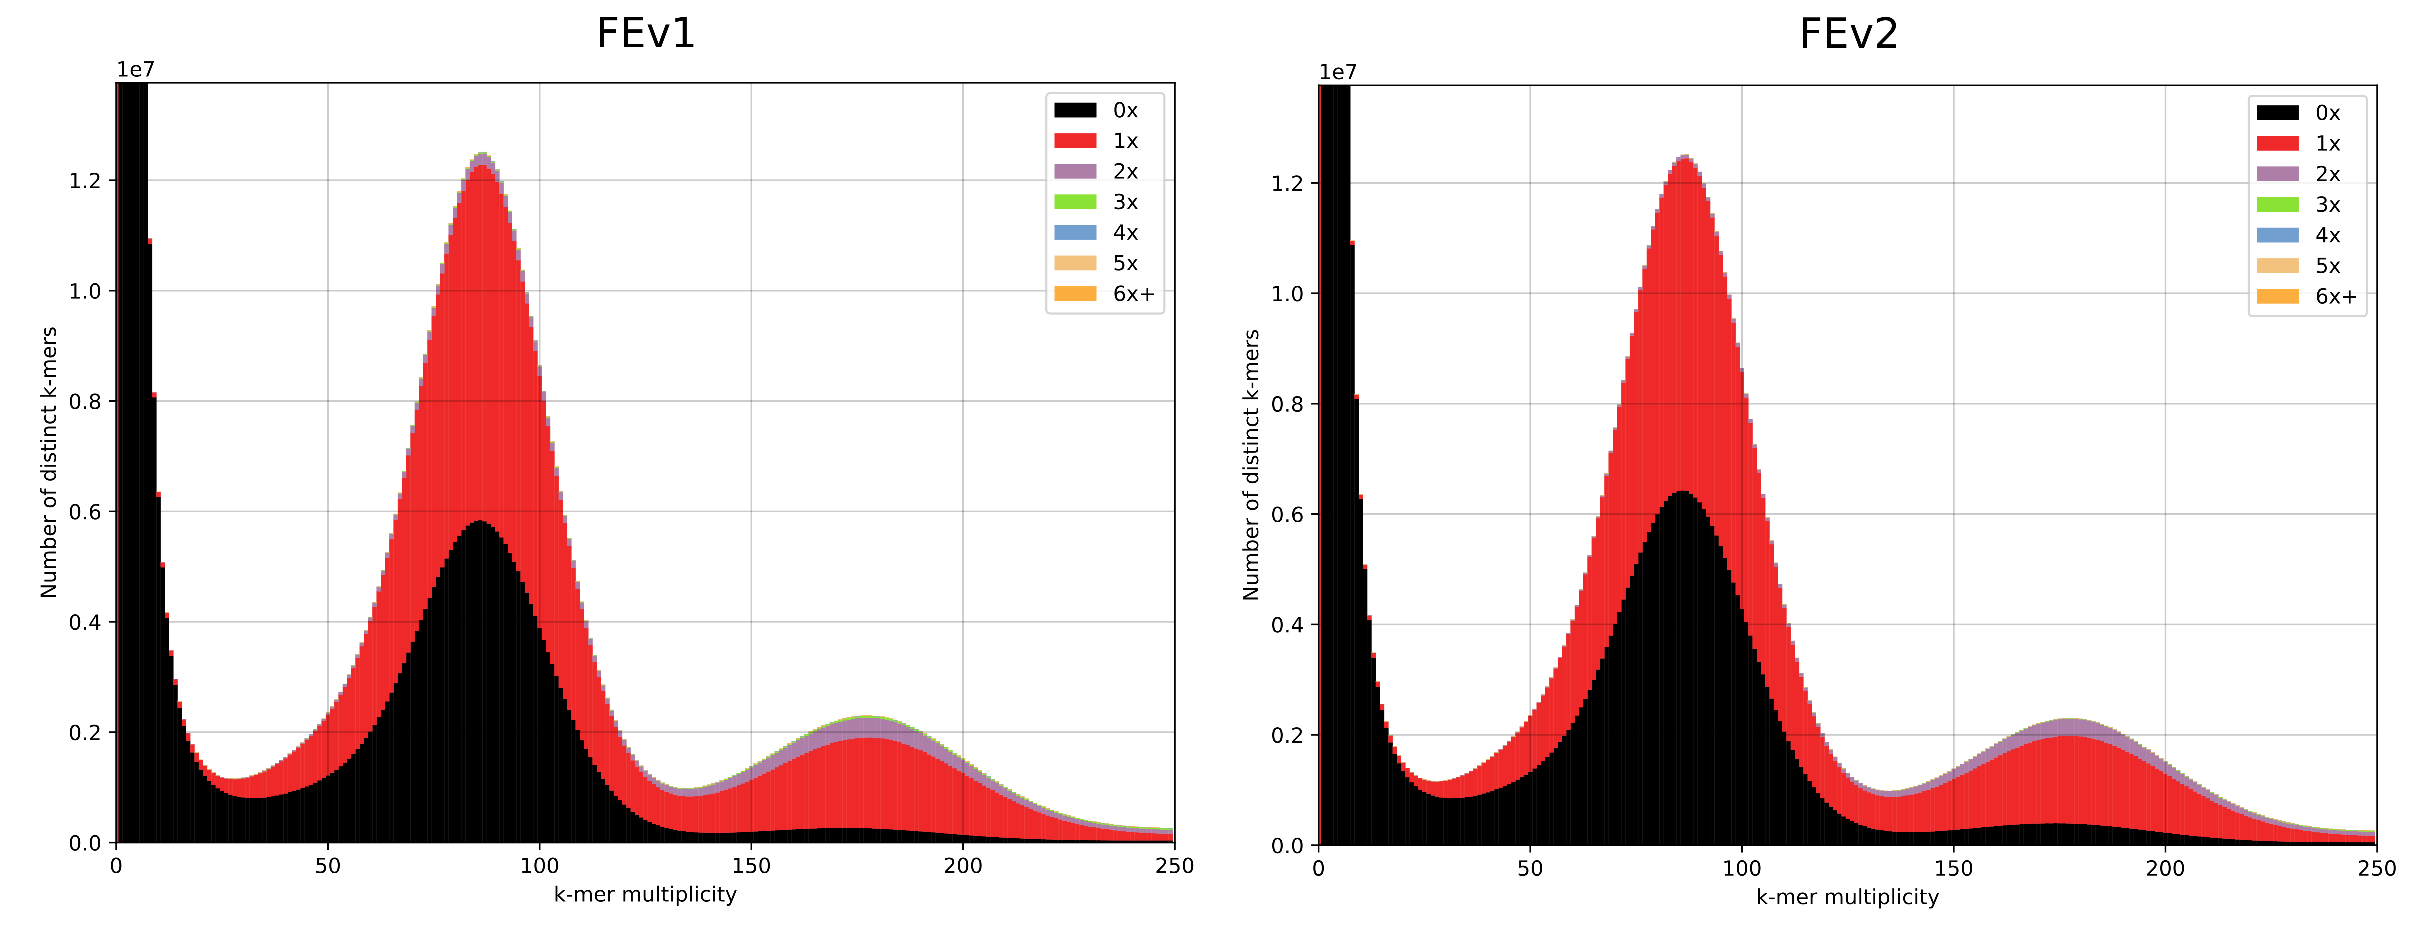
\includegraphics[width=1\linewidth]{fig/fenflata_kat_scaffolded.eps}
    \caption{\textit{k}-mer analysis of chromosome-level scaffolds for the two Hi-C scaffolded assemblies.}
    \label{fig:fenflata_kat_comp}
\end{figure}

\section{Discussion}

The genome of \textit{Flaccisagitta enflata} posed a challenge on several aspects. The amount of DNA that could be extracted from one specimen was too low to run all analysis on a single individual, but it was however sufficient to avoid pooling individuals for long-read sequencing or for Hi-C sequencing. First analysis showed that it was even more desirable to assemble the contigs from only one individual as the genome has a high heterozygosity; thus, a pool of highly divergent individuals would have further hindered the assembly. Using a second individual for Hi-C sequencing is a likely cause for the low mapping rate, due to the variability from one specimen to another. Besides, the collapsed assembly only represents one haplotype for all heterozygous regions; as this genome has a high heterozygosity, many Hi-C reads may fail to map to the missing haplotypes. Considering the level of heterozygosity, a diploid assembly would have been a more complete representation. Such assembly is possible when combining short and long reads, as for the Ratatosk-Canu assembly, but phasing with Hi-C is impossible in this case as the datasets were generated from different specimens. \\

Despite these difficulties, the FEv1 and FEv2 assemblies reached high contiguity and completeness. The draft long-read assemblies had a relatively small N50, which may be to the numerous heterozygous regions causing unresolved bubbles in the assembly graphs and leading to breaks. Still, Hi-C scaffolding with instaGRAAL brought these assemblies to chromosome level; although no karyotype is available for this species, FEv1 and FEv2 both converged towards 9 chromosome-level scaffolds. The assembly is currently under annotation, and will subsequently be analyzed to bring insights into the phylogeny of chaetognaths. \\

This study will serve as a basis for chaetognath genomics, since this is the first chaetognath assembly. Future phylogenomic analyses may shed light on the puzzling position of this clade, and bring insights into its evolution. In addition, the methods used for this project should facilitate new chaetognaths assemblies as it provides resources for high-molecular-weight DNA extraction, Nanopore sequencing, Hi-C sequencing, and assembly.